\documentclass[border=0.2cm]{standalone}
 
\renewcommand{\ttdefault}{pcr}
\renewcommand{\sfdefault}{phv}
\renewcommand{\familydefault}{\sfdefault}
\usepackage[style=english]{csquotes}

\usepackage[dvipsnames]{xcolor}

% Required packages
\usepackage{tikz}
\usetikzlibrary{shapes,positioning}

%% FORMDEFINITIONEN
%% -------------------------------------------------------
% PROZESSSTART
\tikzset{boxTerminator/.style={draw,fill=red!50,rounded rectangle,align=center,font=\footnotesize}}

% PROZESSVORGANG
\tikzset{boxOperation/.style={draw,align=center,font=\footnotesize}}

% PROZESSINPUT/OUTPUT
\tikzset{boxInOutput/.style={draw,fill=blue!20,trapezium,trapezium left angle = 65, trapezium right angle = 115,trapezium stretches,align=left,font=\footnotesize}}

% PROZESSENTSCHEIDUNG
\tikzset{boxDecision/.style={draw,fill=green!30,diamond,aspect=4,%minimum width=2.5cm,
		inner sep=2pt,align=center,font=\footnotesize}}
 
% UNTERPROZESS
% Die Standard-Flowchart-Form für einen Unterprozess gibt es so nicht
% und muss erst neu definiert werden über drei einzelnen Rechtecke nebeneinander
\newcommand{\subprocess}[3]{
% Middle rectangle
\node[boxOperation,fill=yellow!30,outer sep=0,#1,align=center,font=\footnotesize] (#2) {#3};
% Left restangle
\fill[draw,thick,fill=yellow!30] (#2.north west) -- ++ (-0.3,0) |- (#2.south west);
% Right rectangle
\fill[draw,thick,fill=yellow!30] (#2.north east) -- ++ (0.3,0) |- (#2.south east);
}
%% -------------------------------------------------------



\begin{document}
 
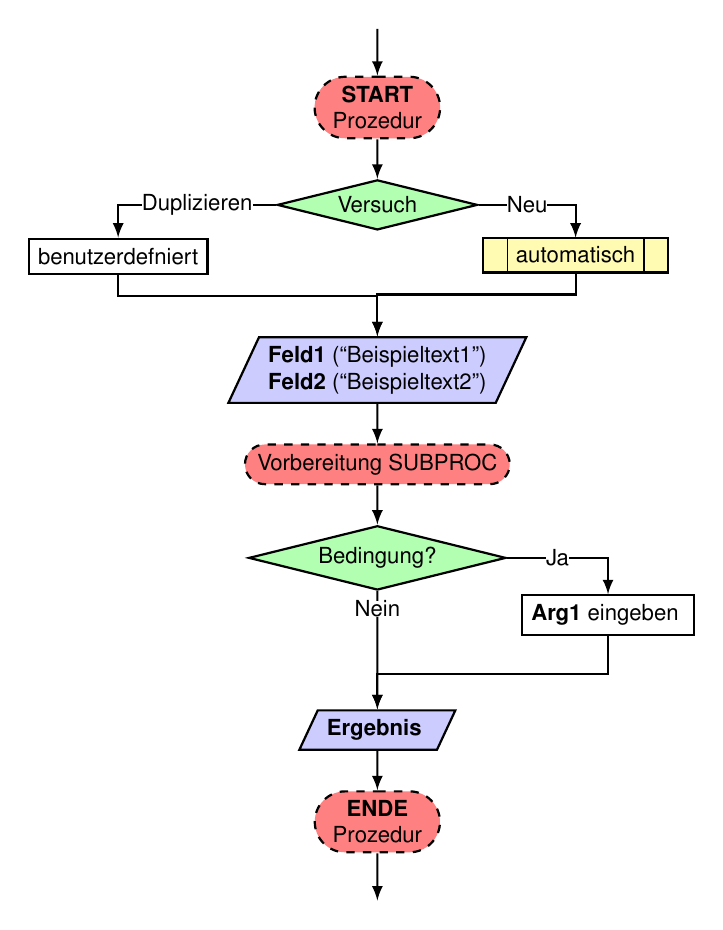
\begin{tikzpicture}[font=\footnotesize, thick, node distance = 0.5cm]
 
% START
\node[boxTerminator,dashed] (block1) {\textbf{START}\\Prozedur};

% PFEIL REIN
\draw[latex-] (block1) --+(0,1);

% VERSUCH
\node[boxDecision,below=of block1] (blockVersuch) {Versuch};
\draw[-latex] (block1) edge (blockVersuch);

% VERSUCH > NEU
\subprocess{below right=0.25cm and 1cm of blockVersuch}{block21}{automatisch}
\draw[-latex] (blockVersuch) -| (block21) node[pos=0.25,fill=white,inner sep=0]{Neu};

% VERSUCH > DUPLIZIEREN
\node[boxOperation,below left=0.25cm and 1.5cm of blockVersuch,align=center] (block22) {benutzerdefniert};
\draw[-latex] (blockVersuch) -| (block22) node[pos=0.25,fill=white,inner sep=0]{Duplizieren};

% FELD1, FELD2
\node[boxInOutput,below=2.5cm of block1] (block3) {
	\textbf{Feld1} (\enquote{Beispieltext1})\\
	\textbf{Feld2} (\enquote{Beispieltext2})};
\draw[-latex] (block21) --+(0,-0.5) -| (block3);
\draw[-latex] (block22)  --+(0,-0.5) -|  (block3);
 
 % VORBEREITUNG SUBPROC
\node[boxTerminator,dashed,below=of block3] (block4) {Vorbereitung SUBPROC};
\draw[-latex] (block3) edge (block4);

% BEDINGUNG
\node[boxDecision,below=of block4] (block7) {Bedingung?};
\draw[-latex] (block4) edge (block7);

% ARG1, ARG2
\node[boxOperation,below right=0.25cm and 1cm of block7] (block8) {
	\textbf{Arg1} eingeben
};
\draw[-latex] (block7) -| (block8) node[pos=0.25,fill=white,inner sep=0]{Ja};

% ERGEBNIS
\node[boxInOutput,below=1.5cm of block7] (block17) {
	\textbf{Ergebnis}
};
\draw[-latex] (block7) edge node[pos=0.15,fill=white,inner sep=0]{Nein} (block17);
\draw[-latex] (block8) --+(0,-0.75) -| (block17);

% ENDE
\node[boxTerminator,dashed,below=of block17] (block23) {\textbf{ENDE}\\Prozedur};
\draw[-latex] (block17) edge (block23);

% PFEIL RAUS
\draw[-latex] (block23) --+(0,-1);
\end{tikzpicture}
 
\end{document}